% Options for packages loaded elsewhere
\PassOptionsToPackage{unicode}{hyperref}
\PassOptionsToPackage{hyphens}{url}
%
\documentclass[
  12 pt,
  a4paper,
]{article}
\usepackage{amsmath,amssymb}
\usepackage{setspace}
\usepackage{iftex}
\ifPDFTeX
  \usepackage[T1]{fontenc}
  \usepackage[utf8]{inputenc}
  \usepackage{textcomp} % provide euro and other symbols
\else % if luatex or xetex
  \usepackage{unicode-math} % this also loads fontspec
  \defaultfontfeatures{Scale=MatchLowercase}
  \defaultfontfeatures[\rmfamily]{Ligatures=TeX,Scale=1}
\fi
\usepackage{lmodern}
\ifPDFTeX\else
  % xetex/luatex font selection
  \setmainfont[]{Times New Roman}
\fi
% Use upquote if available, for straight quotes in verbatim environments
\IfFileExists{upquote.sty}{\usepackage{upquote}}{}
\IfFileExists{microtype.sty}{% use microtype if available
  \usepackage[]{microtype}
  \UseMicrotypeSet[protrusion]{basicmath} % disable protrusion for tt fonts
}{}
\makeatletter
\@ifundefined{KOMAClassName}{% if non-KOMA class
  \IfFileExists{parskip.sty}{%
    \usepackage{parskip}
  }{% else
    \setlength{\parindent}{0pt}
    \setlength{\parskip}{6pt plus 2pt minus 1pt}}
}{% if KOMA class
  \KOMAoptions{parskip=half}}
\makeatother
\usepackage{xcolor}
\usepackage[margin=1in]{geometry}
\usepackage{color}
\usepackage{fancyvrb}
\newcommand{\VerbBar}{|}
\newcommand{\VERB}{\Verb[commandchars=\\\{\}]}
\DefineVerbatimEnvironment{Highlighting}{Verbatim}{commandchars=\\\{\}}
% Add ',fontsize=\small' for more characters per line
\usepackage{framed}
\definecolor{shadecolor}{RGB}{248,248,248}
\newenvironment{Shaded}{\begin{snugshade}}{\end{snugshade}}
\newcommand{\AlertTok}[1]{\textcolor[rgb]{0.94,0.16,0.16}{#1}}
\newcommand{\AnnotationTok}[1]{\textcolor[rgb]{0.56,0.35,0.01}{\textbf{\textit{#1}}}}
\newcommand{\AttributeTok}[1]{\textcolor[rgb]{0.13,0.29,0.53}{#1}}
\newcommand{\BaseNTok}[1]{\textcolor[rgb]{0.00,0.00,0.81}{#1}}
\newcommand{\BuiltInTok}[1]{#1}
\newcommand{\CharTok}[1]{\textcolor[rgb]{0.31,0.60,0.02}{#1}}
\newcommand{\CommentTok}[1]{\textcolor[rgb]{0.56,0.35,0.01}{\textit{#1}}}
\newcommand{\CommentVarTok}[1]{\textcolor[rgb]{0.56,0.35,0.01}{\textbf{\textit{#1}}}}
\newcommand{\ConstantTok}[1]{\textcolor[rgb]{0.56,0.35,0.01}{#1}}
\newcommand{\ControlFlowTok}[1]{\textcolor[rgb]{0.13,0.29,0.53}{\textbf{#1}}}
\newcommand{\DataTypeTok}[1]{\textcolor[rgb]{0.13,0.29,0.53}{#1}}
\newcommand{\DecValTok}[1]{\textcolor[rgb]{0.00,0.00,0.81}{#1}}
\newcommand{\DocumentationTok}[1]{\textcolor[rgb]{0.56,0.35,0.01}{\textbf{\textit{#1}}}}
\newcommand{\ErrorTok}[1]{\textcolor[rgb]{0.64,0.00,0.00}{\textbf{#1}}}
\newcommand{\ExtensionTok}[1]{#1}
\newcommand{\FloatTok}[1]{\textcolor[rgb]{0.00,0.00,0.81}{#1}}
\newcommand{\FunctionTok}[1]{\textcolor[rgb]{0.13,0.29,0.53}{\textbf{#1}}}
\newcommand{\ImportTok}[1]{#1}
\newcommand{\InformationTok}[1]{\textcolor[rgb]{0.56,0.35,0.01}{\textbf{\textit{#1}}}}
\newcommand{\KeywordTok}[1]{\textcolor[rgb]{0.13,0.29,0.53}{\textbf{#1}}}
\newcommand{\NormalTok}[1]{#1}
\newcommand{\OperatorTok}[1]{\textcolor[rgb]{0.81,0.36,0.00}{\textbf{#1}}}
\newcommand{\OtherTok}[1]{\textcolor[rgb]{0.56,0.35,0.01}{#1}}
\newcommand{\PreprocessorTok}[1]{\textcolor[rgb]{0.56,0.35,0.01}{\textit{#1}}}
\newcommand{\RegionMarkerTok}[1]{#1}
\newcommand{\SpecialCharTok}[1]{\textcolor[rgb]{0.81,0.36,0.00}{\textbf{#1}}}
\newcommand{\SpecialStringTok}[1]{\textcolor[rgb]{0.31,0.60,0.02}{#1}}
\newcommand{\StringTok}[1]{\textcolor[rgb]{0.31,0.60,0.02}{#1}}
\newcommand{\VariableTok}[1]{\textcolor[rgb]{0.00,0.00,0.00}{#1}}
\newcommand{\VerbatimStringTok}[1]{\textcolor[rgb]{0.31,0.60,0.02}{#1}}
\newcommand{\WarningTok}[1]{\textcolor[rgb]{0.56,0.35,0.01}{\textbf{\textit{#1}}}}
\usepackage{graphicx}
\makeatletter
\def\maxwidth{\ifdim\Gin@nat@width>\linewidth\linewidth\else\Gin@nat@width\fi}
\def\maxheight{\ifdim\Gin@nat@height>\textheight\textheight\else\Gin@nat@height\fi}
\makeatother
% Scale images if necessary, so that they will not overflow the page
% margins by default, and it is still possible to overwrite the defaults
% using explicit options in \includegraphics[width, height, ...]{}
\setkeys{Gin}{width=\maxwidth,height=\maxheight,keepaspectratio}
% Set default figure placement to htbp
\makeatletter
\def\fps@figure{htbp}
\makeatother
\setlength{\emergencystretch}{3em} % prevent overfull lines
\providecommand{\tightlist}{%
  \setlength{\itemsep}{0pt}\setlength{\parskip}{0pt}}
\setcounter{secnumdepth}{-\maxdimen} % remove section numbering
\ifLuaTeX
\usepackage[bidi=basic]{babel}
\else
\usepackage[bidi=default]{babel}
\fi
\babelprovide[main,import]{spanish}
\ifPDFTeX
\else
\babelfont{rm}[]{Times New Roman}
\fi
% get rid of language-specific shorthands (see #6817):
\let\LanguageShortHands\languageshorthands
\def\languageshorthands#1{}
\ifLuaTeX
  \usepackage{selnolig}  % disable illegal ligatures
\fi
\usepackage{bookmark}
\IfFileExists{xurl.sty}{\usepackage{xurl}}{} % add URL line breaks if available
\urlstyle{same}
\hypersetup{
  pdflang={es-ES},
  hidelinks,
  pdfcreator={LaTeX via pandoc}}

\title{U8 PREPARAR PENDRIVE PER INSTAL·LAR. VENTOY}
\usepackage{etoolbox}
\makeatletter
\providecommand{\subtitle}[1]{% add subtitle to \maketitle
  \apptocmd{\@title}{\par {\large #1 \par}}{}{}
}
\makeatother
\subtitle{Resum característiques}
\author{}
\date{\vspace{-2.5em}}

\begin{document}
\maketitle

\setstretch{1.5}
\newpage

\renewcommand\tablename{Tabla}

\section{1. Introducció}\label{introducciuxf3}

\subsection{1.1 Què és Ventoy}\label{quuxe8-uxe9s-ventoy}

\textbf{Ventoy} és una ferramenta lliure i de codi obert que permet
crear un \textbf{USB bootejable} d'una manera molt més senzilla i
eficient que els mètodes tradicionals. A diferència d'altres programes
com Rufus o UNetbootin, Ventoy no requereix que crees un nou USB
bootejable per a cada imatge ISO; en lloc d'això, simplement copies els
fitxers ISO al pendrive i Ventoy els detecta automàticament en el moment
d'arrancar.

En la \textbf{classificació del software} que vam estudiar a principi de
curs, es tractaria d'un \textbf{software de sistema} que actua molt a
prop del firmware (BIOS/UEFI). Concretament és un gestor d'arrancada.

\subsection{1.2 Característiques principals de
Ventoy}\label{caracteruxedstiques-principals-de-ventoy}

\begin{itemize}
\tightlist
\item
  No cal tornar a formatar el pendrive cada vegada que vols afegir una
  nova ISO.
\item
  Compatible amb BIOS i UEFI sense necessitat de canviar configuracions.
\item
  Suporta múltiples ISOs al mateix USB (pots tenir Linux, Windows i
  eines de recuperació o per clonar al mateix pendrive).
\item
  Admet arxius ISO de més de 4GB (ideal per a Windows 11 o Server).
\item
  100\% de codi obert i gratuït, amb suport per a Windows i Linux.
\end{itemize}

\begin{center}\rule{0.5\linewidth}{0.5pt}\end{center}

\newpage

\section{2. Preparar Ventoy en un pendrive des
d'Ubuntu}\label{preparar-ventoy-en-un-pendrive-des-dubuntu}

\subsection{2.1 Formatejar el pendrive en
NTFS}\label{formatejar-el-pendrive-en-ntfs}

Usem NTFS que admet fitxer amb tamańy superior a 4Gb i compatibilitat en
Windows i Linux

\begin{figure}
\centering
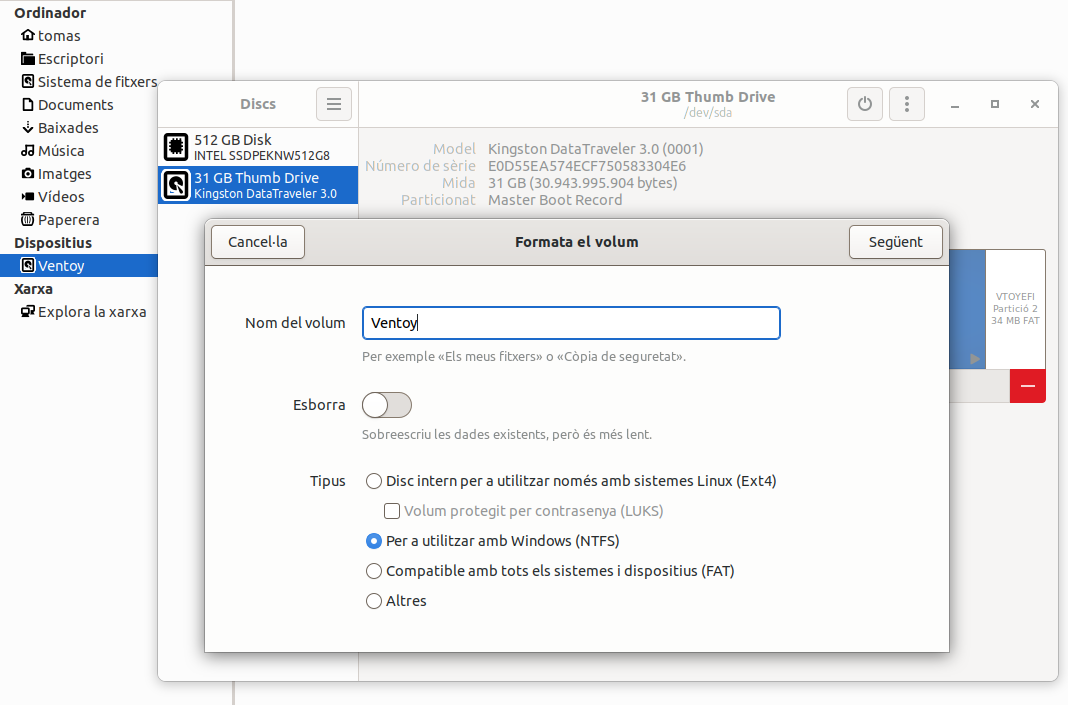
\includegraphics{png/formatar.png}
\caption{Imatge1: Formatejar}
\end{figure}

\subsection{2.2 Descarregar Ventoy}\label{descarregar-ventoy}

Baixa l'última versió de Ventoy per a Linux des del seu web oficial:

\begin{verbatim}
https://www.ventoy.net/en/download.html
\end{verbatim}

Descarrega el fitxer .tar.gz per a Linux. Observeru el codi
\emph{sha256} !

\begin{figure}
\centering
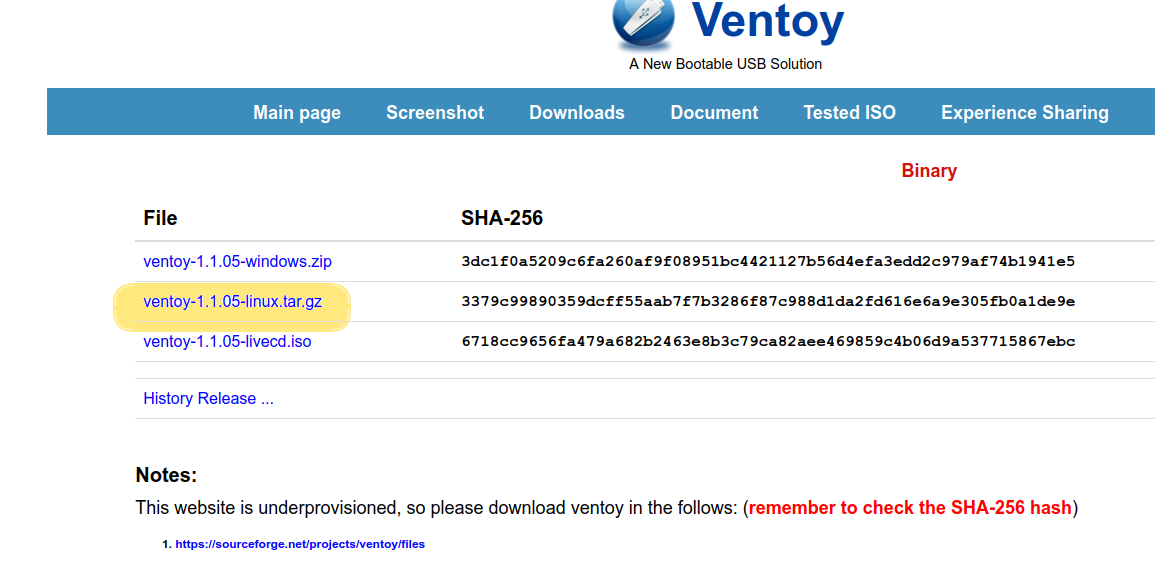
\includegraphics{png/descarrega1.png}
\caption{Imatge2: Descàrrega Ventoy per a Ubuntu}
\end{figure}

Ens obri una segona pàgina des d'on descarregar ja.

\begin{figure}
\centering
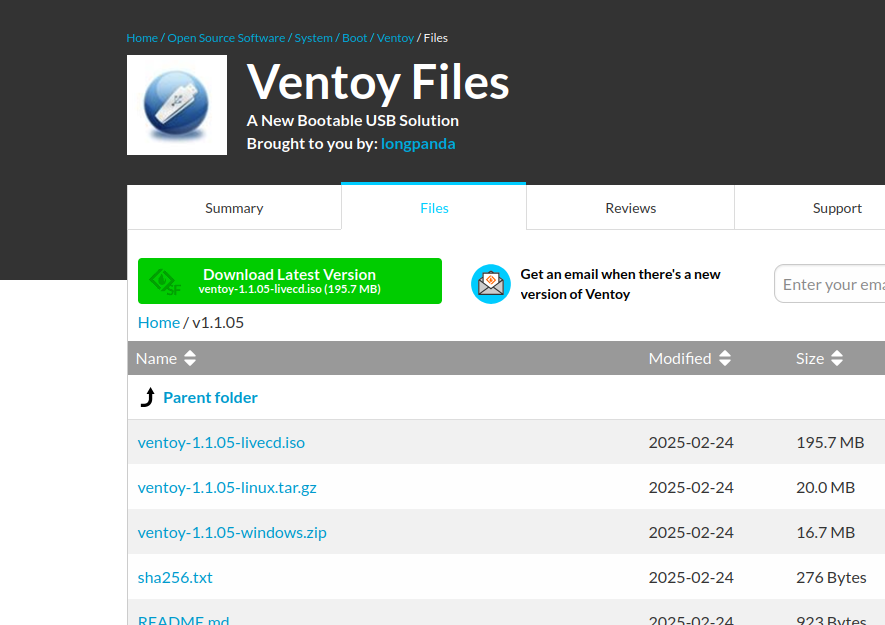
\includegraphics{png/descarrega2.png}
\caption{Imatge3: Descàrrega Ventoy per a Ubuntu}
\end{figure}

\subsubsection{2.2.1 Comprovació
sha256sum}\label{comprovaciuxf3-sha256sum}

Opcionalment podem comprovar si s'ha descarregat bé el fitxer. A la web
de descàrrega esn faciliten el codi sha256 per a comprovar. Executem la
utilitat de Linux i mirem si el valor és igual.

\begin{figure}
\centering
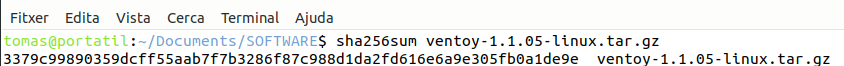
\includegraphics{png/sha256sum.png}
\caption{Imatge3: Comprovació amb sha256sum}
\end{figure}

\subsection{2.3 Extraure l'arxiu}\label{extraure-larxiu}

Obre un terminal i executa:

\begin{Shaded}
\begin{Highlighting}[]
\BuiltInTok{cd}\NormalTok{ \textasciitilde{}/Baixades}
\FunctionTok{tar} \AttributeTok{{-}xvf}\NormalTok{ ventoy{-}}\PreprocessorTok{*}\NormalTok{.tar.gz}
\BuiltInTok{cd}\NormalTok{ ventoy{-}}\PreprocessorTok{*}
\end{Highlighting}
\end{Shaded}

\subsection{2.4 Identificar el dispositiu
USB}\label{identificar-el-dispositiu-usb}

Connecta el teu USB i comprova la seva identificació amb:

\begin{Shaded}
\begin{Highlighting}[]
\ExtensionTok{lsblk}
\end{Highlighting}
\end{Shaded}

O també amb:

\begin{Shaded}
\begin{Highlighting}[]
\FunctionTok{sudo}\NormalTok{ fdisk }\AttributeTok{{-}l}
\end{Highlighting}
\end{Shaded}

Busca el nom del teu USB, per exemple /dev/sdX (substitueix ``X'' per la
lletra correcta).

\subsection{2.5 Instal·lar Ventoy al
pendrive}\label{installar-ventoy-al-pendrive}

Executa la instal·lació (substitueix X per la lletra del teu USB):

\begin{Shaded}
\begin{Highlighting}[]
\FunctionTok{sudo}\NormalTok{ ./Ventoy2Disk.sh }\AttributeTok{{-}i}\NormalTok{ /dev/sdX}
\end{Highlighting}
\end{Shaded}

Això esborrarà tot el contingut del pendrive!

Si vols actualitzar Ventoy sense esborrar dades, usa:

\begin{Shaded}
\begin{Highlighting}[]
\FunctionTok{sudo}\NormalTok{ ./Ventoy2Disk.sh }\AttributeTok{{-}u}\NormalTok{ /dev/sdX}
\end{Highlighting}
\end{Shaded}

Per instal·lar amb confirmació prèvia:

\begin{Shaded}
\begin{Highlighting}[]
\FunctionTok{sudo}\NormalTok{ ./Ventoy2Disk.sh }\AttributeTok{{-}I}\NormalTok{ /dev/sdX}
\end{Highlighting}
\end{Shaded}

\subsection{2.6 Copiar les ISOs al
pendrive}\label{copiar-les-isos-al-pendrive}

Una vegada instal·lat, només cal que copieu les imatges ISO (Windows,
Linux, etc.) directament al pendrive, sense necessitat de crear
particions ni fer res més.

\subsection{2.7 Provar el pendrive}\label{provar-el-pendrive}

\begin{enumerate}
\def\labelenumi{\arabic{enumi}.}
\tightlist
\item
  Reinicia el teu ordinador.\\
\item
  Entra a la BIOS/UEFI prement una de les tecles següents (depèn del
  fabricant):

  \begin{itemize}
  \tightlist
  \item
    F2, F12, ESC, DEL\\
  \end{itemize}
\item
  Canvia l'ordre (BOOT ORDER, BOOT SEQUENCE\ldots) i reodrena pera que
  el pendrive USB siga el 1r dispositiu d'arrencada.
\item
  Reininicia el PC. Si tot ha anat bé, apareixerà el menú de Ventoy amb
  les ISOs que has copiat.
\end{enumerate}

\begin{center}\rule{0.5\linewidth}{0.5pt}\end{center}

\newpage

\section{3. Guia per instal·lar Ventoy en un USB des de Windows
11}\label{guia-per-installar-ventoy-en-un-usb-des-de-windows-11}

\subsection{3.0 Formatar el pendrive}\label{formatar-el-pendrive}

Seleccionem el PenDrive

\begin{figure}
\centering
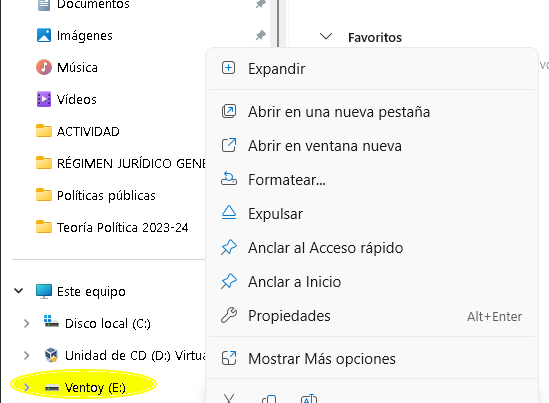
\includegraphics{png/formatWindows.png}
\caption{Imatge 4:Formatejar un Pendrive}
\end{figure}

Indiquem el tipus de Sistema de Fitxers (File System, SF): NTFS

\begin{figure}
\centering
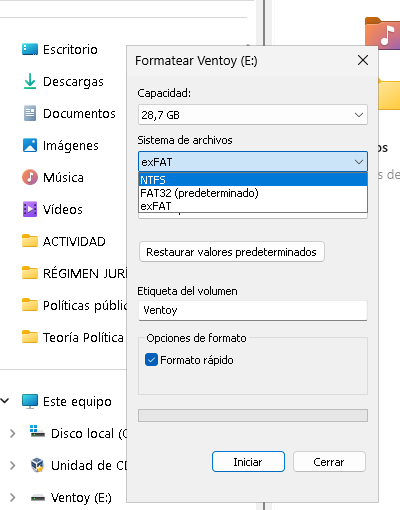
\includegraphics{png/formatWindows2.png}
\caption{Imatge 5:Formatejar un Pendrive:NTFS}
\end{figure}

\subsection{3.1 Descarregar Ventoy per a
Windows}\label{descarregar-ventoy-per-a-windows}

\begin{itemize}
\item
  Ves a la web oficial:\\
  \url{https://www.ventoy.net/en/download.html}
\item
  Descarrega l'arxiu ``Ventoy-xxxxx-windows.zip''.
\end{itemize}

\begin{figure}
\centering
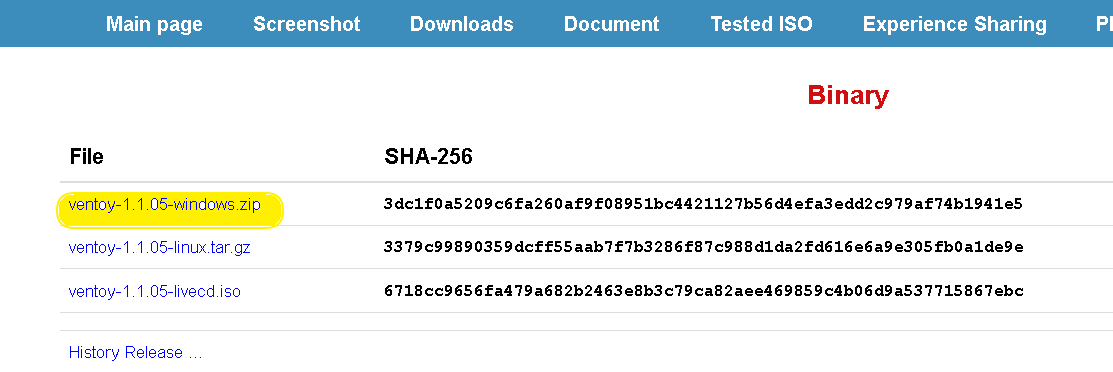
\includegraphics{png/zipDownload.png}
\caption{Imatge 6:Formatejar un Pendrive:NTFS}
\end{figure}

\subsection{3.2 Comprovar el SHA256 del fitxer descarregat
(OPCIONAL)}\label{comprovar-el-sha256-del-fitxer-descarregat-opcional}

Abans d'instal·lar Ventoy, és recomanable comprovar la seva integritat
verificant el \textbf{SHA256} del fitxer descarregat.

\subsubsection{Opció 1: amb PowerShell:
**}\label{opciuxf3-1-amb-powershell}

\begin{enumerate}
\def\labelenumi{\arabic{enumi}.}
\tightlist
\item
  Obri PowerShell (Win + X → Terminal (PowerShell)).\\
\item
  Executa el següent cmdLet:
\end{enumerate}

\begin{Shaded}
\begin{Highlighting}[]
\NormalTok{Get{-}FileHash }\StringTok{"C:\textbackslash{}ruta\textbackslash{}al\textbackslash{}fitxer.zip"} \OperatorTok{{-}}\NormalTok{Algorithm SHA256}
\end{Highlighting}
\end{Shaded}

\begin{enumerate}
\def\labelenumi{\arabic{enumi}.}
\setcounter{enumi}{2}
\tightlist
\item
  Es mostrarà un codi hash. Compara'l amb el proporcionat a la web
  oficial de Ventoy.
\end{enumerate}

\begin{figure}
\centering
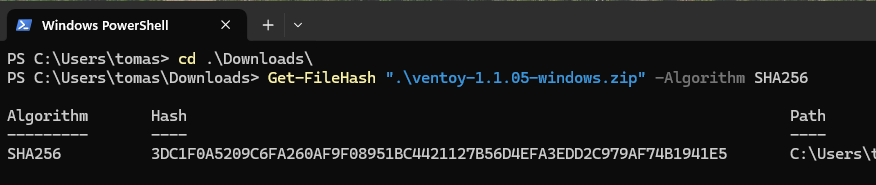
\includegraphics{png/Get-FileHash.png}
\caption{Imatge 6: Get-FileHash}
\end{figure}

\subsubsection{Opció 2: amb CMD
(CertUtil):}\label{opciuxf3-2-amb-cmd-certutil}

\begin{enumerate}
\def\labelenumi{\arabic{enumi}.}
\tightlist
\item
  Obri el símbol del sistema (Win + R, escriu \texttt{cmd} i prem
  Enter).\\
\item
  Escriu la següent ordre:
\end{enumerate}

\begin{Shaded}
\begin{Highlighting}[]
\NormalTok{   certutil }\AttributeTok{{-}hashfile} \StringTok{"C:\textbackslash{}ruta\textbackslash{}al\textbackslash{}fitxer.zip"}\NormalTok{ SHA256}
\end{Highlighting}
\end{Shaded}

\begin{enumerate}
\def\labelenumi{\arabic{enumi}.}
\setcounter{enumi}{2}
\tightlist
\item
  Compara el resultat amb el hash oficial.
\end{enumerate}

\begin{figure}
\centering
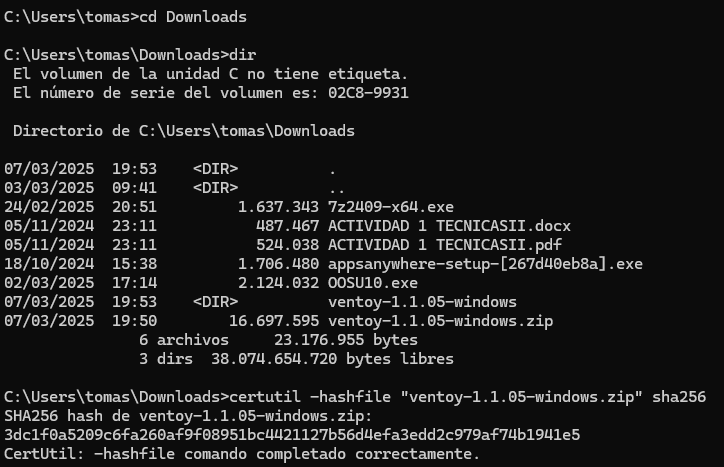
\includegraphics{png/certutil.png}
\caption{Figura 7: certutil}
\end{figure}

\subsection{3.3 Extraure l'arxiu}\label{extraure-larxiu-1}

\begin{enumerate}
\def\labelenumi{\arabic{enumi}.}
\tightlist
\item
  Ves a la carpeta de Descàrregues.\\
\item
  Fes clic dret al fitxer ZIP i selecciona ``Extreure tot\ldots{}''.\\
\item
  Obri la carpeta generada després de l'extracció.
\end{enumerate}

\begin{figure}
\centering
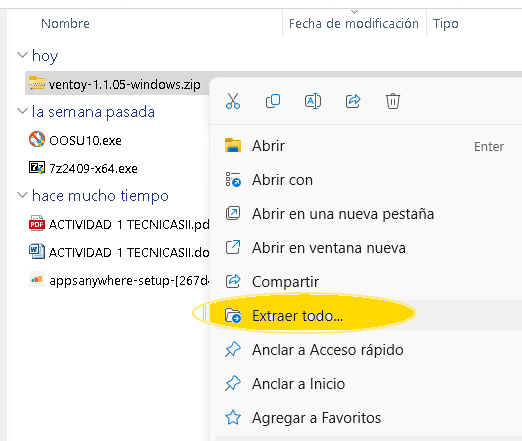
\includegraphics{png/extraerZip.png}
\caption{Imatge 8:Descomprimir ZIP}
\end{figure}

\subsubsection{3.5 Obrir Ventoy}\label{obrir-ventoy}

A la carpeta extreta, \textbf{executa com a Administrador} l'executable
\textbf{Ventoy2Disk.exe}.

\begin{figure}
\centering
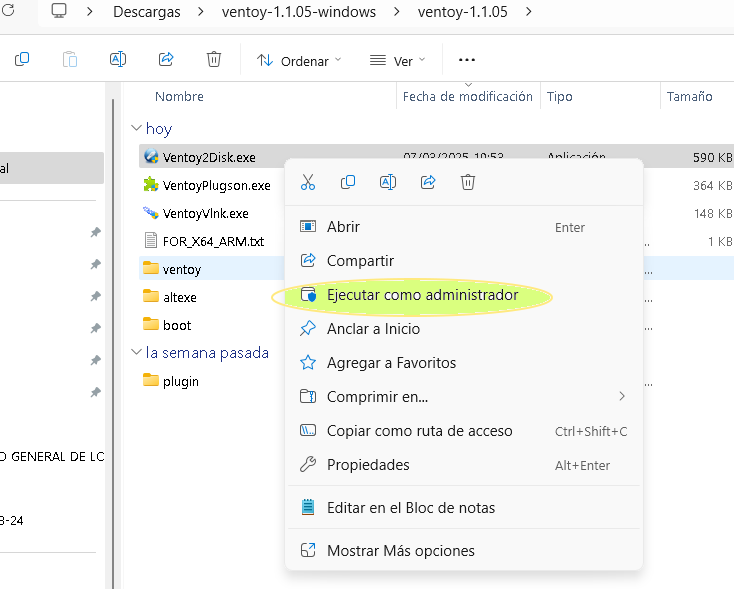
\includegraphics{png/Executar.png}
\caption{Imatge 9: Instal·lar Ventoy des de Windows}
\end{figure}

\subsubsection{3.6 Seleccionar el pendrive i instal·lar
Ventoy}\label{seleccionar-el-pendrive-i-installar-ventoy}

\begin{enumerate}
\def\labelenumi{\arabic{enumi}.}
\tightlist
\item
  A la part superior, assegura't que el dispositiu seleccionat és el teu
  pendrive.\\
\item
  Opcional: Pots clicar a ``Opcions'' → ``Estil de partició'' i escollir
  entre:

  \begin{itemize}
  \tightlist
  \item
    \textbf{MBR} (recomanat per compatibilitat universal, BIOS +
    UEFI).\\
  \item
    \textbf{GPT} (per a UEFI moderns).\\
  \end{itemize}
\item
  Finalment, fes clic a ``Instal·lar''.\\
\item
  Apareixeran dos missatges d'advertència, fes clic a ``Sí'' dues
  vegades per confirmar.
\end{enumerate}

\begin{figure}
\centering
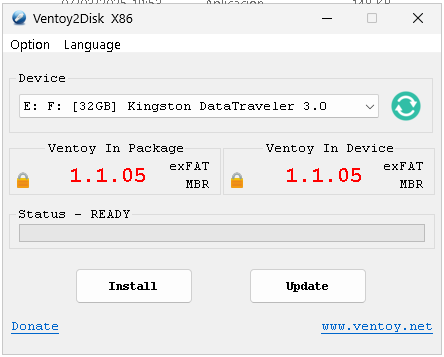
\includegraphics{png/executar2.png}
\caption{Imatge 19: Elegir unitat destí (Pendrive)}
\end{figure}

\begin{figure}
\centering
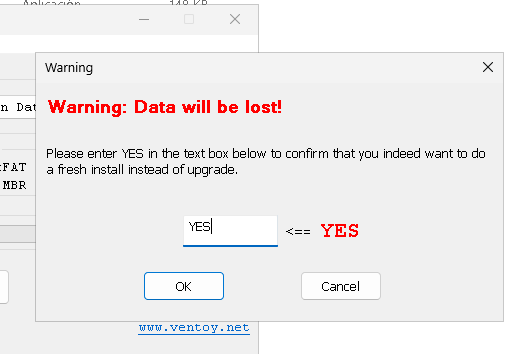
\includegraphics{png/executar3.png}
\caption{Imatge 11: Confirmar instal·lació}
\end{figure}

\subsection{3.7 Copiar les imatges ISO}\label{copiar-les-imatges-iso}

Una vegada instal·lat el Ventoy al Pendrive només cal copiar els fitxers
ISO (per exemple, Windows, Linux, etc.) directament al pendrive.

\subsubsection{3.8 Provar l'arrencada}\label{provar-larrencada}

\begin{enumerate}
\def\labelenumi{\arabic{enumi}.}
\tightlist
\item
  Reinicia el teu ordinador.\\
\item
  Entra a la BIOS/UEFI prement una de les tecles següents (depèn del
  fabricant):

  \begin{itemize}
  \tightlist
  \item
    F2, F12, ESC, DEL\\
  \end{itemize}
\item
  Canvia l'ordre (BOOT ORDER, BOOT SEQUENCE\ldots) i reodrena pera que
  el pendrive USB siga el 1r dispositiu d'arrencada.
\item
  Reininicia el PC. Si tot ha anat bé, apareixerà el menú de Ventoy amb
  les ISOs que has copiat.
\end{enumerate}

\end{document}
